\documentclass{beamer}
\usepackage[utf8]{inputenc}
\usetheme{Copenhagen}
%\usepackage[spanish]{babel}
\usepackage{multirow}
%\usepackage{estilo-apuntes}
\usepackage{braids}
\usepackage[]{graphicx}
\usepackage{rotating}
\usepackage{pgf,tikz}
\usepackage{pgfplots}
\usepackage{tikz-cd}
\usepackage{mathtools}
%\usepackage{oplotsymbl} %filled pentagon go brrrr
%\usepackage{empheq}
%\usepackage[dvipsnames]{xcolor}
%\usepackage{xcolor}

\usetikzlibrary{arrows}
\usetikzlibrary{cd}
\usetikzlibrary{babel}
\pgfplotsset{compat=1.13}
\usetikzlibrary{decorations.shapes}
%\pgfkeyssetvalue{/tikz/braid height}{1cm} %no parece hacer nada
%\pgfkeyssetvalue{/tikz/braid width}{1cm}
%\pgfkeyssetvalue{/tikz/braid start}{(0,0)}
%\pgfkeyssetvalue{/tikz/braid colour}{black}

\theoremstyle{definition}

\newtheorem{theo}{Theorem}
\newtheorem{defi}{Definition}
\newtheorem{prop}[theo]{Proposition}
\newtheorem{lem}[theo]{Lemma}

\newcommand{\Z}{\mathbb{Z}}
\newcommand{\Q}{\mathbb{Q}}
\newcommand{\C}{\mathbb{C}}
\newcommand{\CC}{\mathcal{C}}
\newcommand{\OO}{\mathcal{O}}
\newcommand{\Tot}{\mathrm{Tot}}
\newcommand{\D}{\mathbb{D}}
\newcommand{\s}{\mathfrak{s}}
\providecommand{\gene}[1]{\langle{#1}\rangle}

\DeclareMathOperator{\im}{im}
\DeclareMathOperator{\End}{End}

\addtobeamertemplate{navigation symbols}{}{%
    \usebeamerfont{footline}%
    \usebeamercolor[fg]{footline}%
    \hspace{1em}%
    %\insertframenumber/\inserttotalframenumber
}
\setbeamercolor{footline}{fg=black}
\setbeamerfont{footline}{series=\bfseries}

\newcommand{\highlight}[1]{%
	\colorbox{red!50}{$\displaystyle#1$}}

\makeatletter
%\newcommand*{\encircled}[1]{\relax\ifmmode\mathpalette\@encircled@math{#1}\else\@encircled{#1}\fi}
%\newcommand*{\@encircled@math}[2]{\@encircled{$\m@th#1#2$}}
%\newcommand*{\@encircled}[1]{%
%	\tikz[baseline,anchor=base]{\node[draw,circle,outer sep=0pt,inner sep=.2ex] {#1};}}
%\makeatother


%-----------------------------------------------------------

\title{The derived Deligne conjecture}
\author{Javier Aguilar Mart\'in}
\institute{University of Kent}
\date{}
 
\begin{document}
\frame{\titlepage}


\section{Algebraic Deligne Conjecture}
\begin{frame}
\begin{itemize}
\item<1-> Let $\OO$ be an operad, e.g. $\OO(n)=\End_A(n)=\hom_R(A^{\otimes n},A)$.  %if you know about operads this is obvious, but I want to avoid them
\item<2-> For $f\in \OO(n)$ and $g_i\in \OO(m_i)$ define the \emph{brace} $b_j(f;g_1,\dots, g_j) \in \OO(n+\sum m_i-j)$ as
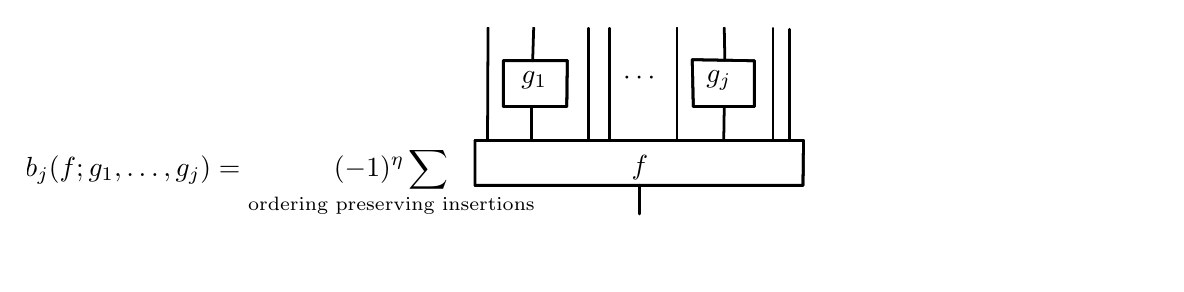
\begin{tikzpicture}[line cap=round,line join=round,>=triangle 45,x=1.0cm,y=1.0cm]
		\clip(-2.8466666666666676,-1) rectangle (11.486666666666668,2.);
		\draw[line width=1.pt] (2.833333333333334,0.) -- (2.833333333333334,0.5666666666666675) -- (7.006666666666668,0.5666666666666675) -- (7.,0.) -- cycle;
		\draw[line width=1.pt] (3.193333333333334,1.) -- (4.,1.) -- (4.006666666666668,1.58) -- (3.193333333333334,1.58) -- cycle;
		\draw[line width=1.pt] (6.,1.) -- (6.38,1.) -- (6.38,1.58) -- (5.593333333333335,1.5933333333333344) -- (5.606666666666667,1.) -- cycle;
		\draw (-3.,0.6) node[anchor=north west] {$b_j(f;g_1,\dots, g_j)=\displaystyle{\underset{\text{ordering preserving insertions}}{(-1)^\eta\sum}}$};
		\draw [line width=1.pt] (2.833333333333334,0.)-- (2.833333333333334,0.5666666666666675);
		\draw [line width=1.pt] (2.833333333333334,0.5666666666666675)-- (7.006666666666668,0.5666666666666675);
		\draw [line width=1.pt] (7.006666666666668,0.5666666666666675)-- (7.,0.);
		\draw [line width=1.pt] (7.,0.)-- (2.833333333333334,0.);
		\draw [line width=1.pt] (4.92,0.)-- (4.92,-0.36666666666666614);
		\draw [line width=1.pt] (2.993333333333334,0.5666666666666675)-- (3.,2.);
		\draw [line width=1.pt] (3.553333333333334,0.5666666666666675)-- (3.553333333333334,1.);
		\draw [line width=1.pt] (4.273333333333334,0.5666666666666675)-- (4.273333333333334,1.9933333333333345);
		\draw [line width=1.pt] (4.54,0.5666666666666675)-- (4.54,1.9933333333333345);
		\draw [line width=1.pt] (5.993333333333334,0.5666666666666675)-- (6.,1.);
		\draw [line width=1.pt] (6.62,0.5666666666666675)-- (6.62,1.9933333333333345);
		\draw [line width=1.pt] (6.833333333333335,0.5666666666666675)-- (6.833333333333335,1.98);
		\draw [line width=1.pt] (3.193333333333334,1.)-- (4.,1.);
		\draw [line width=1.pt] (4.,1.)-- (4.006666666666668,1.58);
		\draw [line width=1.pt] (4.006666666666668,1.58)-- (3.193333333333334,1.58);
		\draw [line width=1.pt] (3.193333333333334,1.58)-- (3.193333333333334,1.);
		\draw [line width=1.pt] (6.,1.)-- (6.38,1.);
		\draw [line width=1.pt] (6.38,1.)-- (6.38,1.58);
		\draw [line width=1.pt] (6.38,1.58)-- (5.593333333333335,1.5933333333333344);
		\draw [line width=1.pt] (5.593333333333335,1.5933333333333344)-- (5.606666666666667,1.);
		\draw [line width=1.pt] (5.606666666666667,1.)-- (6.,1.);
		\draw [line width=1.pt] (3.5666666666666673,1.58)-- (3.58,2.);
		\draw [line width=1.pt] (6.007451656136321,1.586314378709553)-- (6.,2.);
		\draw [line width=1.pt] (5.4,0.5666666666666675)-- (5.4,2.);
		\draw (3.3,1.5666666666666678) node[anchor=north west] {$g_1$};
		\draw (5.65,1.58) node[anchor=north west] {$g_j$};
		\draw (4.7,0.5) node[anchor=north west] {$f$};
		\draw (4.59,1.5533333333333343) node[anchor=north west] {$\cdots$};
		\end{tikzpicture}
\item<3-> Notation: $b_1(f;g)=f\circ g = \sum_i f\circ_i g$.
\end{itemize}
\end{frame}

\subsection{Hochschild complex}
\begin{frame}
\frametitle{Hochschild complex of an associative algebra}
For $f\in \End_A(n)$ let $|f|=\deg(f)+n$.\pause
\begin{lem}
The operation $[f,g]=f\circ g-(-1)^{|f|-1}g\circ f$ defines a Lie bracket on $\End_A$. 
\end{lem}\pause

\begin{defi}
Let $A$ be a dg algebra. Its \emph{Hochschild complex} $\End_A$ is given by $\End_A(n)=\hom_R(A^{\otimes n},A)$ with the differential %I like C^0 as R -> A
\[
D(f) = [d+m,f] = d\circ f - (-1)^{|f|-1}f\circ d + m\circ f - (-1)^{|f|-1}f\circ m %the jacobi identity guarantees that this is a differential
\]
where $d$ and $m$ are the differential and multiplication on $A$.
\end{defi}

\end{frame}

\begin{frame}
\begin{itemize}
\item $\End_A$ is also a dga with multiplication %so we can consider its Hochschild complex and it has brace structure etc
\[
M(f_1,f_2) = (-1)^{|f|-1}b_2(m;f_1,f_2).
\]
\end{itemize}\pause
\begin{prop}[Gerstenhaber-Voronov]
The map $\End_A\to \End_{\End_A}$ given by 
\[
x\mapsto \sum_{j\geq 0} b_j(x;-)
\]
is a map of dgas.
\end{prop}
\end{frame}


\subsection{Deligne conjecture}
\begin{frame}
\frametitle{Algebraic Deligne conjecture}
%When you unravel what the above means
\begin{theo}[Gerstenhaber-Voronov]
 The Hochschild complex $\End_A$ has the structure of a \emph{homotopy $G$-algebra}:\pause
 \begin{align*}
 b_j(m(f_1,&f_2);g_1,\dots,g_j) = \\
 &\sum_{k=0}^j (-1)^\varepsilon m(b_k(f_1;g_1,\dots, g_k),b_{j-k}(f_2;g_{k+1},\dots, g_j))
 \end{align*}
 %varepsilon is the koszul sign
 and
\end{theo}
\end{frame}
\begin{frame}
\begin{block}{}
 \begin{align*}
&b_j(D(f);g_1,\dots, g_j)-D(b_j(f;g_1,\dots,g_j))\\
-&(-1)^{|f|+1}\sum_{p=1}^j(-1)^{\sum_{i=1}^p|g_i|}b_j(f;g_1,\dots,D(g_p),\dots, g_j)\\
=&-(-1)^{(|f|+1)|g_1|}M(g_1,b_{j-1}(f;g_2,\dots, g_j))\\
 &+(-1)^{|f|+1}\sum_{p=1}^{j-1}(-1)^{j-1+\underset{i=1}{\overset{p}{\sum}}|g_i|}b_{j-1}(f;g_1,\dots,M(g_p,g_{p+1}),\dots g_j)\\
 &-(-1)^{|f|+\sum_{i=1}^{j-1}|g_i|}M(b_{j-1}(f;g_1,\dots, g_{j-1}),g_j)
\end{align*}
\end{block}
\end{frame}


\section{$A_\infty$-algebras}


\begin{frame}
\frametitle{$A_\infty$-algebras}
\begin{defi}
An $A_\infty$-\emph{algebra} $A$ is an $R$-module equipped with a family of ``multiplications'' $m_n:A^{\otimes n}\to A$ of degree $2-n$ satisfying the relation %MAYBE CHANGE CHAINS TO COCHAINS TO KEEP THE DEGREE 2-N, I WILL HAVE TO USE OPERADIC DESUSPENSION IN THIS CASE

\[\sum_{r+s+t\geq 1}(-1)^{rs+t}m_{r+1+t}(1^{\otimes r}\otimes m_s\otimes 1^{\otimes s})=0\] %we are composing every map with itself
\end{defi}
\end{frame}


\begin{frame}
\frametitle{Some particular cases}
\begin{itemize}
\item<1-> We always have $m_1m_1=0$, so in particular $A$ is a cochain complex.%CAN BE DEFINED ON THE CATEGORY OF CHAIN COMPLEX
\item<2-> If $m_i=0$ for $i\neq 2$, the relation becomes $m_2(1\otimes m_2)=m_2(m_2\otimes 1)$, so $A$ is an associative algebra.
\item<3->  We also have the relation \[m_1m_2=m_2(m_1\otimes 1)+m_2(1\otimes m_1)\]%DG %MONOID IN CHAIN COMPLEX ANALOGUE TO MONOID IN K-VECT
\item[]<4-> This is the Leibniz rule, and $A$ is a dga.
\end{itemize}
\end{frame}


\begin{frame}
\frametitle{$A_\infty$-algebras are homotopy associative algebras.}
%how do they generalize associative algebras
\begin{itemize}
\item<1-> For $r+s+t=3$ we have the relation
\begin{align*}
&m_2(m_2\otimes 1)-m_2(1\otimes m_2)=\\ %the failure of m_2 to be associative
&m_1m_3+m_3(m_1\otimes 1\otimes 1)+m_3(1\otimes m_1\otimes 1)+m_3(1\otimes 1\otimes m_1)
\end{align*}
\item[]<2-> $m_2$ is homotopy associative with homotopy given by $m_3$. %recall that m1 is a differential so on homology this vanishes
\item<3-> The higher relations are a homotopy coherent extension of this fact. %m3 satisfies some relation up to homotopy given by m4 and so on
\end{itemize}
\end{frame}


\begin{frame}
\frametitle{Morphisms of $A_\infty$-algebras}
\begin{defi}
An \emph{$\infty$-morphism} of $A_\infty$-algebras $A\to B$ is a family of maps \[f_n:A^{\otimes n}\to B\] of degree $1-n$ satisfying for all $n\geq 1$ the equation
\begin{align*}
\sum_{r+s+t=n} (-1)^{rs+t}f_{r+1+t}(1^{\otimes r} \otimes m^A_s\otimes 1^{\otimes t})=\\
\sum_{i_1+\cdots+i_k=n} (-1)^s m^B_k(f_{i_1}\otimes\cdots\otimes f_{i_k}),
\end{align*}
where
$s=\sum_{\alpha<\beta}i_\alpha(1-i_\beta)$.%The composition of $\infty$-morphisms $f:A\to B$ and  $g:B\to C$ is given by 
%
%\[(gf)_n=\sum_r\sum_{i_1+\cdots+i_r=n}(-1)^s g_r(f_{i_1}\otimes\cdots
%\otimes f_{i_r}).\]
\end{defi}

\end{frame}
\begin{frame}
\begin{itemize}
\item<1-> We have $f_1m_1 = m_1f_1$, i.e. $f_1$ is a morphism of complexes.
\item<2-> We have
\[
f_1m_2 = m_2 (f_1\otimes f_1) + m_1f_2 + f_2 (m_1\otimes 1 + 1\otimes m_1),\]
which means that $f_1$ commutes with the multiplication $m_2$ up to a homotopy
given by $f_2$.
\end{itemize}
\end{frame}

\subsection{Minimal models}
\begin{frame}
\frametitle{Minimal models}
\begin{itemize}
\item An $A_\infty$-algebra is \emph{minimal} if $m_1 = 0$. 
\end{itemize}\pause
\begin{theorem}[Kadeishvili]
\begin{itemize}
\item If $A$ is a dga over a field, its cohomology $H^*(A)$ is a minimal $A_\infty$-algebra with multiplication $m_2$ induced by the multiplication on $A$.
\item There is an $\infty$-morphism of $A_\infty$-algebras $f:H^*(A)\to A$ such that $f_1$ is a quasi-isomorphism.
\item Under certain homological conditions, any other dga $A'$ with $H^*(A')\cong H^*(A)$ is quasi-isomorphic to $A$. 
\end{itemize}
\end{theorem}\pause
The $A_\infty$-algebra $H^*(A)$ is called the \emph{minimal model} of $A$. %This will be relevant later
%nice enough = HH(A,A) vanishes on degree 2-n %Replaced  means equivalent  %essentially = up to quasi-iso
%We would like to extend this result to a ground ring that is not necessarily a field.
\end{frame}

\subsection{Operadic Suspension}
\begin{frame}
\frametitle{Operadic suspension}
\begin{itemize}
\item<1-> Define $\Lambda(n)$ to be a 1-dimensional graded module concentrated in degree $n-1$.
\item<2-> The \emph{operadic suspension} $\mathfrak{s}\mathcal{O}$ of an operad $\mathcal{O}$ is given by $\mathfrak{s}\mathcal{O}(n)=\mathcal{O}(n)\otimes \Lambda(n)$ and composition maps determined by the following fact %grading here is deg + arity - 1
\item[]<3->
\begin{theorem}[Markl]
There is an isomorphism of operads
\[ \mathfrak{s}End_{S A}\cong End_A\]
\end{theorem}
%\item<1-> Let $\Lambda(n)$ be a graded vector space concentrated in degree $1-n$ and generated by $e^n=e_1\land\cdots\land e_n$.
%\item<2-> Consider the sign action of the permutation group on $e^n$:
%\[(i\ i+1)\cdot e^n=e_l\land\cdots\land e_{i+1}\land e_i\land\cdots\land e_n=-e^n\]
%\item<3-> Define insertion maps $\circ_i:\Lambda(n)\otimes\Lambda(m)\to\Lambda(n+m-1)$ as
%\[(e_1\land\cdots\land e_n)\otimes(e_1\land\cdots\land e_m)\mapsto  (-1)^{(n-i)(1-m)}e_1\land\cdots\land e_{n+m-1}\]
%\item[]<4-> \[e^n\circ_i e^m= (-1)^{(n-i)(1-m)}e^{m+n-1}\]
\end{itemize}
\end{frame}

\begin{frame}
\begin{itemize}

\item<1-> We may identify each $x\in\mathcal{O}(n)$ with $x\otimes e^n\in \mathfrak{s}\mathcal{O}(n)$.
%\item<2-> If $x$ has degree $p$ in $\mathcal{O}$, it has degree $p-n+1$ in $\mathfrak{s}\mathcal{O}$.
\item<2-> Let $\circ_i$ be the $i$-th insertion on $\mathcal{O}$ and $\tilde{\circ}_i$ the $i$-th insertion on $\mathfrak{s}\mathcal{O}$ then
\[a\tilde{\circ}_ib=(-1)^{(n-1)\deg(b)+(n-i)(m-1)}a\circ_i b.\]
\item<3-> Applied to $A_\infty$-maps 
\[m_{r+1+t}\tilde{\circ}_{r+1}m_s=(-1)^{rs+t}m_{r+1+t}\circ_{r+1}m_s\]
\item[]<4-> The sign of the $A_\infty$-equation!
\end{itemize}
\end{frame}

\begin{frame}
\begin{itemize}
\item<1-> This simplifies the equation to
\[\sum_{r+s+t=n}m_{r+1+t}\tilde{\circ}_{r+1}m_s=0\] %but we can simplify it even more
\item<2-> Let $a\tilde{\circ}b=\sum_{i}a\tilde{\circ}_ib$ and let $m=m_1+m_2+\cdots$. The equation becomes just
\item[]<3-> \[m\tilde{\circ}m=0.\]
\end{itemize}
\end{frame}
\subsection{Hochschild complex}

\begin{frame}
Let $\OO=\End_A$.
\begin{itemize}
\item<1-> Since $m\tilde{\circ}m=0$, the Jacobi identity implies that $[m,[m,]]=0$ for the bracket induced by $\tilde{\circ}$.
\item<2-> Since $|m|=1$, the map $[m,]:\s\OO\to \s\OO$ turns $\s\OO$ into a cochain complex.
\item<3-> Indeed, it is possible to define an $A_\infty$-algebra structure on $S\s\OO$. 
\end{itemize}
\end{frame}
\begin{frame}
\frametitle{$A_\infty$-multiplications}
\begin{prop}[Getzler]
Up to shifts, the following maps define an $A_\infty$-algebra structure on $S\s\OO$
\begin{align*}
&M_1(f)=[m,f]\\ %some shifts are omitted
&M_j(f_1,\dots, f_j)=\tilde{b}_j(m;f_1,\dots, f_j) %the brace induced by the new circle
\end{align*}
%generalices the associative result
\end{prop}\pause

\begin{prop}[Hinted at by Gerstenhaber-Voronov]
The map $\Phi:S\s\End_A\to S\s\End_{S\s\End_A}$ given by $\Phi(x)= \sum_{j\geq 0} \tilde{b}_j(x;-)$ satisfies for all $j$
\[\Phi(M_j) = M_j(\Phi^{\otimes j})\]
%generalices the associative result
\end{prop}
\end{frame}


\subsection{Deligne conjecture}
\begin{frame}
\frametitle{$A_\infty$-Deligne conjecture}
\begin{theorem} %some structure was already known, but no complete set of brace relations 
The Hochschild complex $S\s\End_A$ has the structure of a \emph{$J$-algebra}:
\begin{align*}
\tilde{b}_n&(M_j(f_1,\dots, f_j);g_1,\dots, g_n)=\\
&\sum_{\mathclap{l,i_1,k_1,\dots, i_j,k_j}}(-1)^{\varepsilon}M_l(g_1,\dots, \tilde{b}_{k_1}(f_1;g_{i_1},\dots),\dots, \tilde{b}_{k_j}(f_j;g_{i_j},\dots),\dots, g_n).\\ 
\\
&\tilde{b}_j(M_1(f);g_1,\dots, g_j)=\\
&\sum_{l,k,i_1}(-1)^{\varepsilon}M_l(g_1,\dots, \tilde{b}_{k}(f;g_{i_1},\dots),\dots, g_j)\\
&-(-1)^{|f|-1}\sum_{l,k,i_1} (-1)^{\eta} \tilde{b}_k(f;g_1,\dots, M_l(g_{i_1},\dots,), \dots, g_j)
\end{align*}
\end{theorem}
\end{frame}

\section{Derived $A_\infty$-algebras}

\begin{frame}
\frametitle{Derived $A_\infty$-algebras}
\begin{defi}
  A \emph{derived $A_\infty$-algebra} on a $(\Z,\Z)$-bigraded $R$-module $A$ consist of a family of $R$-linear maps 
\[m_{ij}:A^{\otimes j}\to A\]
of bidegree $(i,2-(i+j))$ for each $j\geq 1$, $i\geq 0$, satisfying the equation
\begin{equation*}
\underset{j=r+1+t}{\sum_{\mathclap{u=i+p, v=j+q-1}}}(-1)^{rq+t+pj}m_{ij}(1^{\otimes r}\otimes m_{pq}\otimes 1^{\otimes t})=0
\end{equation*}
for all $u\geq 0$ and $v\geq 1$. 
\end{defi}
\end{frame}

\begin{frame}
\frametitle{Particular cases}
\begin{itemize}
\item<1-> A $dA_\infty$-algebra where $m_{ij}=0$ for all $i>0$ is an $A_\infty$-algebra.
\item<2-> A $dA_\infty$-algebra with $m_{ij}=0$ except for for $m_{01}$ and $m_{11}$ is a \emph{bicomplex}: 
\[m_{01}m_{01}=0,\ m_{11}m_{11}=0,\ m_{01}m_{11}=m_{11}m_{01}\]
\item<3-> A \emph{bidga} is a monoid in the category of bicomplexes, equivalently, a $dA_\infty$-algebra with $m_{ij}=0$ for $i+j\geq 3$.
\end{itemize}
\end{frame}

\begin{frame}
\begin{defi}
Let $A$ and $B$ be derived $A_\infty$-algebras with respective structure maps $m^A$ and $m^B$. An \emph{$\infty$-morphism of derived $A_\infty$-algebras} $f:A\to B$ is a family of maps $f_{st}:A^{\otimes t}\to B$ of bidegree $(s,1-s-t)$ satisfying
\begin{align*}
\underset{j=r+1+t}{\sum_{u=i+p, v=j+q-1}}(-1)^{rq+t+pj}f_{ij}(1^{\otimes r}\otimes m_{pq}^A\otimes 1^{\otimes s})=\\
\underset{v=q_1+\cdots +q_j}{\sum_{u=i+p_1+\cdots +p_j}}(-1)^{\epsilon} m^B_{ij}(f_{p_1 q_1}\otimes\cdots\otimes f_{p_j q_j})
\end{align*}
for all $u\geq 0$ and $v\geq 1$, where
$\epsilon = u + \sum_{1\leq w < l \leq j} q_w(1-p_l-q_l)  + \sum_{w=1}^j p_w(j-w)$.
%I am confindent that this is the same as in RW, it is a matter of grouping differently (taking in to account how many times things are added up) and sometimes change w by j-w. But maybe I should write it down.
\end{defi}
\end{frame}

\begin{frame}
\frametitle{$E_2$-equivalences}
\begin{itemize}
\item<1-> Since $m_{01}m_{01}=0$, denote $H^*_{ver}(A)=H^*(A,m_{01})$. 
\item<2-> Since $m_{21}m_{01} - m_{11}m_{11} + m_{01}m_{21} = 0$, we have that $m_{11}$ is a differential on $H^*_{ver}(A)$. Denote $H^*_{hor}(H^*_{ver}(A)) = H^*(H^*_{ver}(A);m_{11})$.
\end{itemize}\pause
\pause
\begin{defi}
An $\infty$-morphism $f : A \to B$ of derived $A_\infty$-algebras
is called an \emph{$E_2$-equivalence} if $H^*_{hor}(H^*_{ver}(f_{01}))$
is an isomorphism of $R$-modules.
\end{defi}\pause
\begin{defi}
Let $A$ be a dga. A \emph{degreewise $R$-projective
resolution} of $A$ is a degreewise $R$-projective
bidga $P$ with $m_{01} = 0$ together with an $E_2$-equivalence $P \to A$.
\end{defi}
\end{frame}
\subsection{Minimal models}
\begin{frame}
\frametitle{Minimal models}
\begin{itemize}
\item A $dA_\infty$-algebra is \emph{minimal} if $m_{01} = 0$. 
\end{itemize}\pause
\begin{theorem}[Sagave]
Let $A$ be a dga over $R$. Then there is a degreewise
$R$-projective derived $A_\infty$-algebra $E$ together with an $E_2$-equivalence $E \to A$ such that
\begin{itemize}
\item $E$ is minimal,
\item $E$ is well-defined up to $E_2$-equivalence,
\item together with the differential $m_{11}$ and the multiplication $m_{02}$, $E$ is a degreewise $R$-projective
resolution of the graded algebra $H^*(A)$. 
\end{itemize}
\end{theorem}\pause
Such $E$ is called a \emph{minimal model} of $A$.
\end{frame}

\subsection{Totalization}
\begin{frame}
\frametitle{Totalization}
\begin{itemize}
\item<1-> Consider only \emph{bounded on the right} bigraded modules $A$: there exist $i'$ such that $A_i^j=0$ for all $j$ and $i>i'$. %monoidality reasons, not too restrictive in practice
\item<2-> We call $j$ the \emph{vertical degree}, $i$ the \emph{horizontal degree} and $d=i+j$ the \emph{total degree}.
\item[]<3->
\begin{defi}
The \emph{totalization} $\Tot(A)$ of $A = \{A^j_i \}$ is given by
\[\Tot(A)^d =
\bigoplus_{i}A^{d-i}_i \]%\oplus\prod_{i\geq 0}A^{d-i}_i .\]
%The \emph{column filtration} of $\Tot(A)$ is the filtration given by \[F_p\Tot(A)^n \coloneqq\prod_{i\geq p} A^{n-i}_i .\]
\end{defi}\pause
%\item[]<4->
\begin{prop}
$\Tot$ induces a strict monoidal functor with natural transformation $\mu:\Tot(A)\otimes\Tot(B)\to\Tot(A\otimes B)$.
\end{prop}
\end{itemize}
\end{frame}

\subsection{Vertical suspension}

\begin{frame}
\frametitle{Structure on the Hochschild complex}
For a bigraded operad $\OO$ consider the vertical suspension $\s\OO$.
\begin{itemize}
\item<1-> Define $\tilde{\circ}_i$ by considering only vertical degree: for $f\in \OO(n)^j_i$ and $g\in \OO(m)^l_k$
\[f\tilde{\circ}_rg=(-1)^{(n-1)l+(n-r)(m-1)}f\circ_r g.\]
\item<2-> This produces a bigraded Lie bracket $[,]$ and braces $\tilde{b}_j$ that ignore horizontal degrees.

\end{itemize}
\end{frame}

\subsection{Operadic totalization}


\begin{frame}
Let $\Tot(\OO)$ be the totalization of $\OO$.
\begin{itemize}
\item<1-> For $f=\sum_i f_i\in \Tot(\s\OO(n))$ and $g=\sum_i g_i\in \Tot(\s\OO(m))$ define %it has a reason but i'm not talking about operads
\begin{align*}
(f\star_ig)_k&= \Tot(\tilde{\circ}_i)(\mu(f\otimes g))\\
			 &=\sum_{\mathclap{k_1+k_2=k}} (-1)^{(n-1)(\deg(g)-k_2)+(n-i)(m-1)+k_1\deg(g)}f_{k_1}\circ_i g_{k_2}
\end{align*}

\item<2-> If $m=\sum_{i,j} m_{ij}$, then the derived $A_\infty$-equation simplifies to 
\[m\star m = 0.\]
\item<3-> By previous constructions, $\Tot(\End_A)$ is an $A_\infty$-algebra.
\end{itemize}
\end{frame}


\begin{frame}
\frametitle{Connection to $A_\infty$-algebras}
\begin{theorem}[Cirici, Santander, Livernet, Whitehouse]
For a bigraded module $A$ bounded on the right, there is a one to one correspondence between $A_\infty$-algebras on $\Tot(A)$ and $dA_\infty$-algebras on $A$.
\end{theorem}\pause
\begin{corollary}
Up to shifts, the following maps define an $dA_\infty$-algebra structure on $\End_A$
\begin{align*}
&M_{i1}(f)=[m_{i\bullet},f]\\
&M_{ij}(f_1,\dots, f_j)=\tilde{b}_j(m_{i\bullet};f_1,\dots, f_j)
\end{align*}
\end{corollary}

\end{frame}

\begin{frame}
\begin{corollary}
The map $\Phi:S\s\End_A\to S\s\End_{S\s\End_A}$ given by $\Phi(x)= \sum_{j\geq 0} \tilde{b}_j(x;-)$ satisfies for all $j$
\[\Phi(M_{ij}) = M_{ij}(\Phi^{\otimes j})\]
%generalices the associative result
\end{corollary}
\end{frame}

\subsection{Deligne conjecture}
\begin{frame}
\frametitle{Derived Deligne conjecture}
\begin{theorem} %some structure was already known, but no complete set of brace relations 
The Hochschild complex $S\s\End_A$ is a \emph{derived $J$-algebra}:
\begin{align*}
\tilde{b}_n&(M_{ij}(f_1,\dots, f_j);g_1,\dots, g_n)=\\
&\sum_{\mathclap{l,i_1,k_1,\dots, i_j,k_j}}(-1)^{\varepsilon}M_{il}(g_1,\dots, \tilde{b}_{k_1}(f_1;g_{i_1},\dots),\dots, \tilde{b}_{k_j}(f_j;g_{i_j},\dots),\dots, g_n).\\ 
\\
&\tilde{b}_j(M_{i1}(f);g_1,\dots, g_j)=\\
&\sum_{l,k,i_1}(-1)^{\varepsilon}M_{il}(g_1,\dots, \tilde{b}_{k}(f;g_{i_1},\dots),\dots, g_j)\\
&-(-1)^{|f|}\sum_{l,k,i_1} (-1)^{\eta} \tilde{b}_k(f;g_1,\dots, M_{il}(g_{i_1},\dots,), \dots, g_j)
\end{align*}
\end{theorem}
\end{frame}



\begin{frame}
\begin{center}
\Huge{Thank you very much!}
\end{center}
\end{frame}








\end{document}